\section{Discussion}
\label{sec:discussion}

\begin{figure*}
\vskip-5mm
\begin{center}
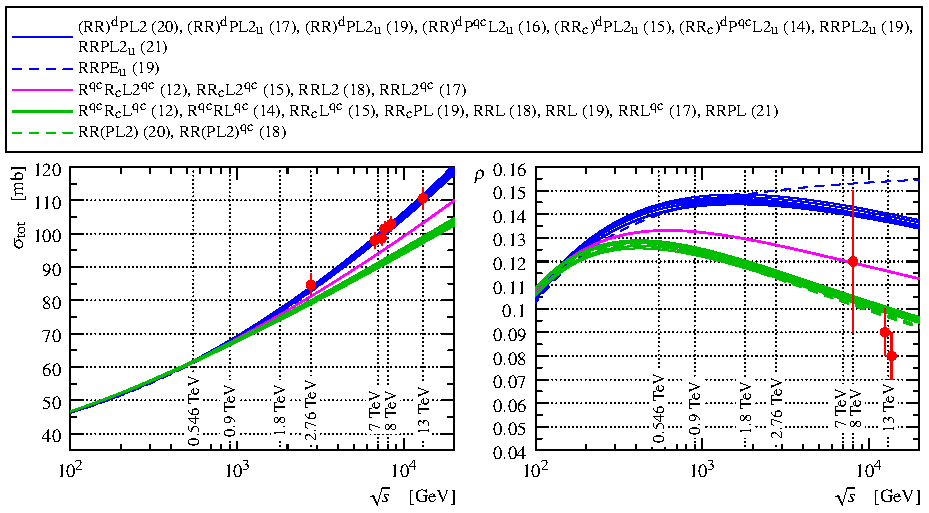
\includegraphics{fig/compete_bands_si_tot_rho.pdf}
\caption{%
Predictions of COMPETE models \cite{compete-details} for $\rm pp$ interactions. Each model is represented by a line (see legend). The red points represent the reference TOTEM measurements. \TODO{add sigma tot determination from this publication ?}
}
\label{fig:comp bands}
\end{center}
\end{figure*}

On of very comprehensive (and therefore representative) studies of the pre-LHC data is by the COMPETE collaboration \cite{compete}. In total 256 models have been considered to describe $\sigma_{\rm tot}$ and $\rho$ data for various reactions ($\rm pp$, $\rm p\pi$, $\rm pK$, etc.) and their anti-reactions. Out of these models, 23 have been found to give reasonable description of the data \cite{compete-details}. These models are confronted with newer TOTEM data in Figure~\ref{fig:comp bands}, showing that the COMPETE models form 3 bands plotted in different colours. While only the blue-band models are compatible with $\sigma_{\rm tot}$ data, for $\rho$ only the green-band models are compatible. Considering the shown five $\sigma_{\rm tot}$ points and two $\rho$ points, the compatibility with the blue band is excluded at \TODO{XXX}, with magenta at \TODO{YYY} and with green at \TODO{ZZZ sigma}. For this calculation, the measurements were considered as independent which can be justified by using data from different LHC fills, using different beam optics, often different energies, often using different RPs, often different analysis approaches (fit parametrisation, treatment of CNI) and often analysed by different teams. In conclusion, none of the COMPETE models is compatible with the ensemble of TOTEM's $\sigma_{\rm tot}$ and $\rho$ measurements.

\bgroup
\parskip=0pt

\> summary/examples of ''common knowledge''
\>> COMPETE
\>>> show that our data are incompatible
\>>> significance 1: si\_tot incompatibility with magenta and green bands; correct the statement of Cudell
\>>> significance 2: rho incompatibility with magenta and blue bands;
\>> something about dispersion relations ??

\> inevitability to modify the current models
\>> at high energies, not many options other than Odderon left to reconcile data with models

\> Odderon
\>> introduced in axiomatic theory: Nicolescu
\>> studied in Regge theory as counter part of Pomeron
\>> inevitable object in QCD 
\>>> bound state of 3 gluons, JPC = 1--
\>>> bound state (with reasonable life time), thus it must be colourless
\>>> bound together more than interactions with other particles
\>>> virtual exchange in t channel, non-perturbative regime
\>>> exists in perturbative calculations
\>>> predicted by lattice calculations: s-channel, name oddball or vector glueball, ground state JPC=1--, our data (indirect) proof of its existence

\> manifestations of Odderon
\>> rho -- why it is interesting
\>> dip region, our 2nd golded channel
\>>> e.g. 62 GeV data, mention this in outlook -- interest to repeat the same at high energy
\>> dip size as function of energy

\> models that can describe the data
\>> Nicolescu
\>> Durham
\>> in both cases Odderon improves agreement with data


\egroup






\begin{figure*}
\vskip-5mm
\begin{center}
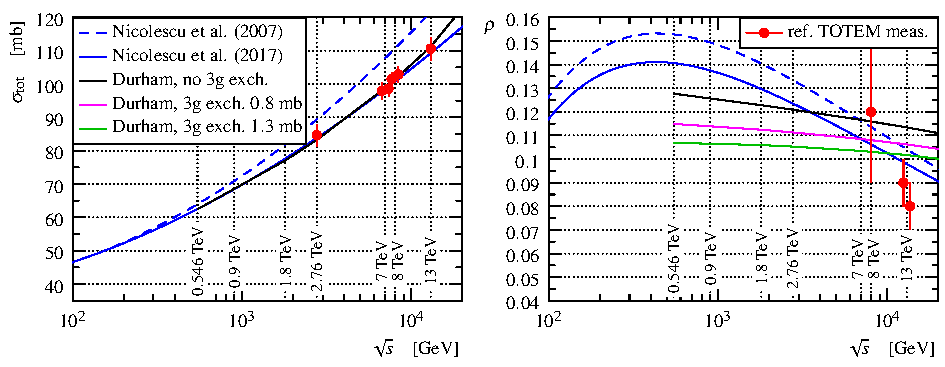
\includegraphics{fig/matching_models_si_tot_rho.pdf}
\caption{%
\TODO{write}
}
\label{fig:match models}
\end{center}
\end{figure*}
